%
% ****
\chapter{Einleitung}
% ****
%
Beginnen Sie jedes Kapitel mit einer kurzen Einleitung die angibt, was
der nachfolgende Text beinhaltet bzw. was die Zielsetzung des Kapitels
ist. Belegen Sie Aussagen durch eigene Entwicklungen, Rechnungen und
Analysen sowie Zitate \cite{NeuronalDynamics}. Verwenden Sie
hierzu $\backslash$\texttt{cite}\{verweis\} und bauen Sie sich
sinnvollerweise eine eigene \textsc{Bib}\TeX-Datei entsprechend dem
Layout in der beiliegenden Datei \texttt{main.bib}.
%
% ***
\section{Allgemeines}
% ***
%
\begin{remark}[Textfluss und mathematische Gleichungen]
  Gleichungen sind Teil des Textes, d.h. Satzzeichen gehen in eine
  Gleichung ein. Zum Beispiel ist die folgende Darstellung
  \textbf{korrekt}.  

  \noindent\textit{Die Lagrange-Funktion ist definiert durch 
  %
  \begin{align}
    L=T-V,
  \end{align}
  %
  wobei $T$ die kinetische Energie und $V$ die potenzielle Energie des
  Systems beschreiben.}

  \noindent \textbf{Nicht korrekt} ist das folgende Beispiel.

  \noindent\textit{Die erste Gleichung ergibt sich aus der Bewegung des Arms.
  %
  \begin{align}
    \dot{x} = f(x,u)
  \end{align}
  %
  Die zweite Gleichung folgt leicht aus der Analyse des
  2. Teilsystems.}

\end{remark}

\begin{remark}[Konventionen und Abkürzungen]
  Es gelten die folgenden Konventionen:
  %
  \begin{itemize}
  \item Skalare Größen $x$
  \item Vektoren $\vec{x}$
  \item Matrizen $A$, Matrizenelemente $A_{i,j}$
  \end{itemize}
  %  
  Darüber hinaus sind die folgenden Befehle vordefiniert
  %
  \begin{itemize}
  \item \matlab als $\backslash$\textsf{matlab} 
  \item \simulink als $\backslash$\textsf{simulink}
  \item \dspace als $\backslash$\textsf{dspace}
  \end{itemize}
  %
  Verweise auf Funktionen von z.B. \matlab werden wie folgt angegeben
  %
  \begin{itemize}
  \item \texttt{ode45} als $\backslash$\texttt{texttt\{ode45\}}
  \end{itemize}
  %
\end{remark}
%
%
%***
\section{Mathematische Formeln}
%***
%
Für $\vec{u}\in\mathds{R}^m$ gelte 
%
\begin{align}
  \label{eq:gleichung1}
  \dot{\vec{x}} &= A \vec{x} + B \vec{u}, && t>0,\quad\vec{x}(0)=\vec{x}_0\\
  \vec{y} &= C\vec{x} + D\vec{u}&& t\geq 0.
\end{align}
%
%
%***
\section{Abbildungen}
%***
%
Eine Abbildung kann wie folgt eingebunden werden: 
%
\begin{verbatim}
\begin{figure}[!h]
  \centering
  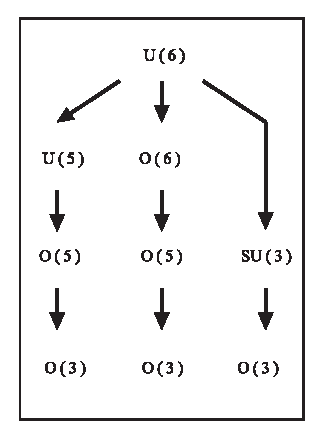
\includegraphics[width=4cm]{figure}
  \caption{Die Bildunterschrift sollte eine sinnvolle Erläuterung der
    Darstellung geben und ist immer mit einem Satzpunkt abzuschließen.}
  \label{fig:abbildung1}
\end{figure}
\end{verbatim}
%
Dies führt auf das folgende Ergebnis:  
%
\begin{figure}[!h] %[!t] ...
  \centering
  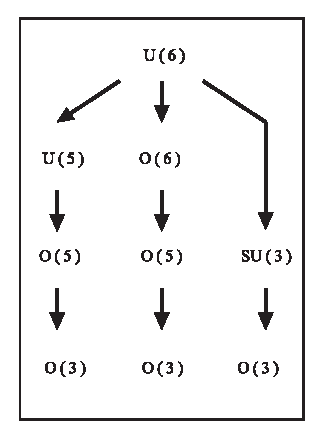
\includegraphics[width=4cm]{figure}
  \caption{Die Bildunterschrift sollte eine sinnvolle Erläuterung der
    Darstellung geben und ist immer mit einem Satzpunkt abzuschließen.}
  \label{fig:abbildung1}
\end{figure}
%

Nutzen Sie bitte ausschließlich die Formate \texttt{.eps} oder
\texttt{.pdf} sowie \texttt{.mps} für Abbildungen. Achten Sie darauf,
dass die Achsenbeschriftung der Textgröße entspricht und lesbar
ist. Verwenden Sie Bildlegenden, die z.B. mittels \matlab erzeugt
werden, eher sparsam. Für eine einzelne Kurve ist keine Legende
notwendig. 
 
%
%***
\section{Textfluss}
%***
%
Gehen Sie sparsam mit Absätzen im Text um. Ein Absatz sollte
ausschließlich durch eines \textbf{Leerzeile} erzeugt
werden. Vermeiden Sie die Verwendung des Befehls
$\backslash\backslash$ zur Erzielung eines manuellen Zeilenumbruchs. 

Neue Absätze werden, im Rahmen dieser Vorlage, durch eine
Einrückung gekennzeichnet. Beachten Sie bitte, dass im Allgemeinen
vor und nach einer Gleichung \textbf{keine} Leerzeile folgen sollte,
da hierdurch unnötige Abstände in den Text integriert werden. 


%%% Local Variables: 
%%% mode: latex
%%% TeX-master: "main"
%%% End: 
